
\chapter{Desarrollo}
\label{cha:desarrollo}

\begin{FraseCelebre}
  \begin{Frase}
    Cada uno de nosotros debe trabajar para su propia mejora, y al mismo tiempo compartir una responsabilidad general para toda la humanidad.
  \end{Frase}
  \begin{Fuente}
    Marie Curie
  \end{Fuente}
\end{FraseCelebre}

\section{Introducción}
\label{sec:intro-desarrollo}

\textcolor{red}{Decir que se ha decidido por emplear algoritmos de detección con redes neuronales convolucionales para abordar los objetivos de este proyecto. Tal como se vió en la sección de conclusiones del capítulo del Estado del Arte se va a Utilizar YOLOv4 junto con DeepSORT para realizar el seguimiento de personas y objetos de interés. Contar que primero se va a probar con Darknet el funcionamiento de YOLOv4 y posteriormente se decide utilizar como framework Tensorflow ya que nos va a facilitar las tareas de programación. Después entrenamiento de la red con el dataset OID para ver si así mejora las métricas de calidad de MS COCO y comparar. Después probar YOLOv4 con Tensorflow convirtiendo el modelo y posteriormente utilizar DeepSORT y filtrar personas y objetos. Finalmente apartado donde se va a ver la estrategia para determinar como identificar un objeto abandonado, esquema del algoritmo e implementación, ya se verá en el apartado de resultados lo que sale.}

\section{YOLOv4}
\label{sec:desarrollo-yolov4}

Darknet es uno de esos marcos de redes neuronales de código abierto escrito en C y CUDA y sirve como base de YOLO. Es rápido, fácil de instalar y admite cálculos de CPU y GPU. Darknet se utiliza como marco para entrenar YOLO, lo que significa que establece la arquitectura de la red. El primer autor de Darknet es el autor del propio YOLO (J Redmon).

\section{Datasets utilizados para el entrenamiento de YOLOv4}
\label{sec:datasets-utilizados}

\subsection{MS COCO Dataset}
\label{subsec:coco-dataset}

\textcolor{red}{El dataset \gls{coco} es gran dataset que contiene más de 200 000 imágenes distribuidas en 80 clases de objetos que representan escenas del mundo real. Se trata de un dataset lo suficientemente grande para que una red bien entrenada sea capaz de aprender características visuales de calidad para el reconocimiento y detección de objetos en imágenes.}

\begin{figure}[ht]
\centering
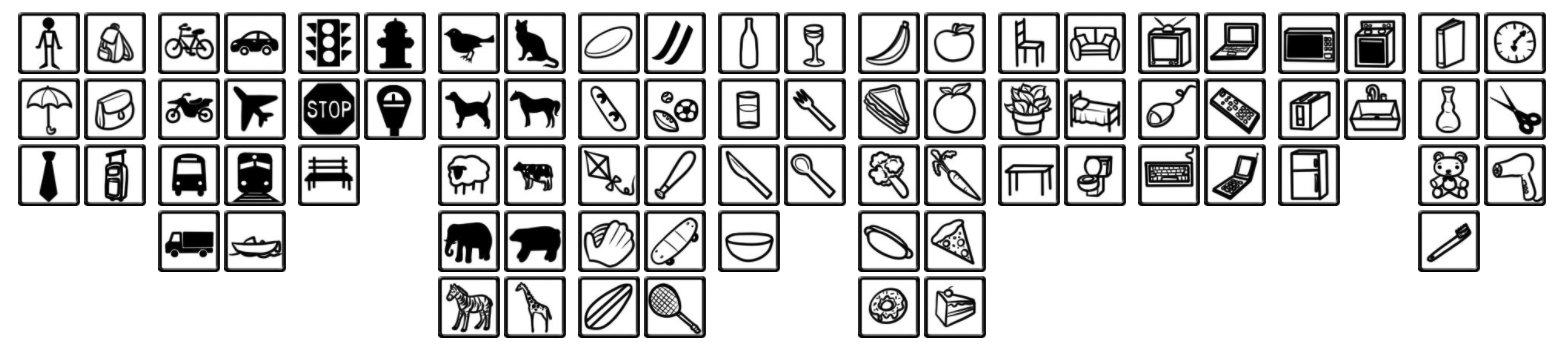
\includegraphics[width=0.9\textwidth]{img/chapters/resultados/datasets/cocodataset.png}
\caption{\label{fig:cocodataset}Categorías de objetos del dataset MS COCO}
\end{figure}

\newpage

\subsection{Open Images Dataset v4}
\label{subsec:OIDv4-dataset}

\begin{figure}[ht]
\centering
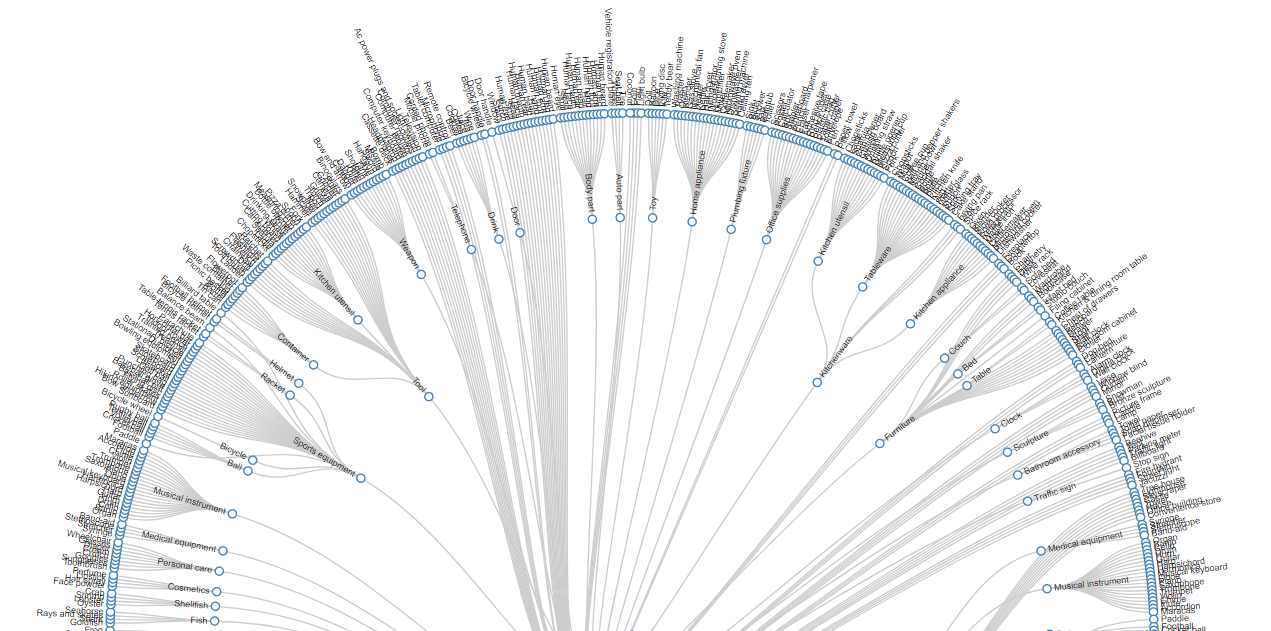
\includegraphics[width=0.7\textwidth]{img/chapters/resultados/datasets/oid-classes.png}
\caption{\label{fig:oiddataset}Categorías de objetos del dataset Open Images Dataset v4}
\end{figure}

\section{Entrenamiento YOLOv4 con Open Image Dataset v4}
\label{sec:train-openimagesv4}

\textcolor{red}{Aquí explicar como he entrenado una red neuronal con otro dataset a partir del repositorio \cite{OIDv4_ToolKit}}

\textcolor{red}{Explicar que se ha tomado 1500 imágenes de entrenamiento de las clases: person, handbag, backpack, suitcase y 300 imágenes de validación.}

\vspace{0.5cm}
\begin{lstlisting}[language=iPython,caption=Descarga dataset Open Images Dataset v4,captionpos=b,label={lst:download-oidv4}]
# Clonar el repositorio de Github
git clone https://github.com/theAIGuysCode/OIDv4_ToolKit.git
cd OIDv4_ToolKit

# Instalacion de las librerias y dependendencias
pip install -r requirements.txt

# Descarga de las imagenes de entrenamiento con un limite de 1500
python main.py downloader --classes Person Handbag Backpack Suitcase --type_csv train --limit 1500 --multiclasses 1

# Descarga de las imagenes de validacion con un limite de 300
python main.py downloader --classes Person Handbag Backpack Suitcase --type_csv validation --limit 300 --multiclasses 1

# Convertir etiquetas al formato de Darknet
python convert_annotations.py

\end{lstlisting}

\begin{figure}[ht]
\centering
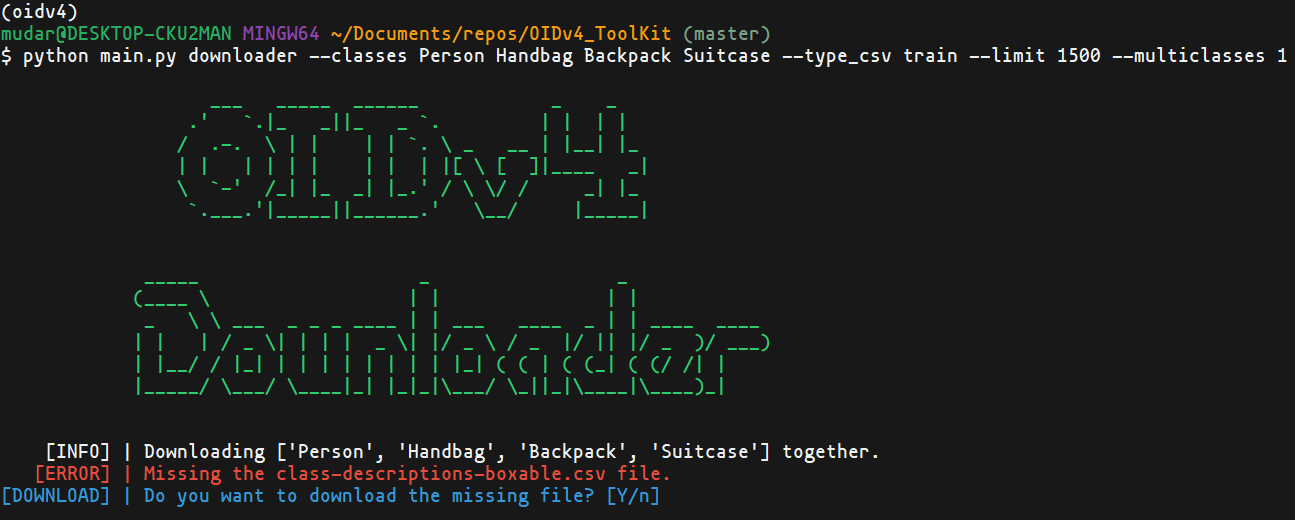
\includegraphics[width=0.3\textwidth]{img/chapters/resultados/datasets/download-oidv4.png}
\caption{\label{fig:download-oidv4}Descarga del dataset Open Images Dataset v4}
\end{figure}

\begin{figure}[ht]
\centering
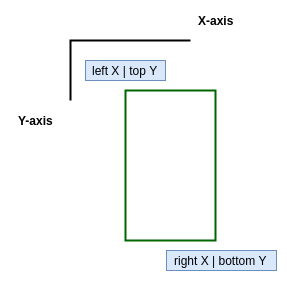
\includegraphics[width=0.3\textwidth]{img/chapters/resultados/datasets/bbox-oidv4.png}
\caption{\label{fig:bbox-oidv4}Estructura de las etiquetas de Open Images Dataset v4}
\end{figure}

La estructura que siguen las etiquetas del dataset de Open Images Dataset v4 es la siguiente:

\texttt{nombre de la clase x left top y x right bottom y}

\aviso{Aquí especificar que se utilizará MS COCO como dataset de entrenamiento de la red y se mostrará los resultados obtenidos de este entrenameinto en el capítulo de resultados}

\newpage

\section{Algoritmo de detección de objetos abandonados}
\label{sec:algoritmo-object-detection}

\textcolor{red}{Dibujar el esquema que voy a seguir para determinar cuando un objeto ha sido abandonado.}
\url{https://app.diagrams.net/}

\newpage

\section{Conclusiones}
\label{sec:conclu-desarrollo}

\begin{algorithm}[H]
 \caption{How to write algorithms}
 \label{alg:howto}
 \KwData{this text}
 \KwResult{how to write algorithm with \LaTeX2e }
 initialization\;
 \While{not at end of this document}{
  read current\;
  \eIf{understand}{
   go to next section\;
   current section becomes this one\;
   }{
   go back to the beginning of current section\;
  }
 }
\end{algorithm}